%!TEX TS-program = xelatex
%!TEX encoding = UTF-8 Unicode

\documentclass[12pt]{extarticle}
% extarticle is like article but can handle 8pt, 9pt, 10pt, 11pt, 12pt, 14pt, 17pt, and 20pt text

\def \ititle {Origins of Mind}
 
\def \isubtitle {Lecture 08}
 
\def \iauthor {Stephen A. Butterfill}
\def \iemail{s.butterfill@warwick.ac.uk}
\date{}

%for strikethrough
\usepackage[normalem]{ulem}

\input{$HOME/Documents/submissions/preamble_steve_handout}

%logic symbol \leftmodels
\usepackage{MnSymbol}

%\bibpunct{}{}{,}{s}{}{,}  %use superscript TICS style bib
%remove hanging indent for TICS style bib
%TODO doesnt work
\setlength{\bibhang}{0em}
%\setlength{\bibsep}{0.5em}


%itemize bullet should be dash
\renewcommand{\labelitemi}{$-$}

\begin{document}

%\raggedcolumns

\begin{multicols*}{3}

\setlength\footnotesep{1em}


\bibliographystyle{newapa} %apalike

%\maketitle
%\tableofcontents




%--------------- 
%--- start paste
\def \ititle {Logic I}
 
\def \isubtitle {Fast Lecture 03}
 
\begin{center}
 
{\Large
 
\textbf{\ititle}: \isubtitle
 
}
 
 
 
\iemail %
 
\end{center}
 
Readings refer to sections of the course textbook, \emph{Language, Proof and Logic}.
 
 
 
\section{What does ‘→’ mean?}
 
\emph{Reading:} §7.1
 
Assuming that the rules of Fitch are such that it is impossible to prove an argument which is not logically valid, the truth table for → is fixed if we accept →Elim and →Intro.
 
How do the rules of proof for → fix its truth table?
 
\begin{center}
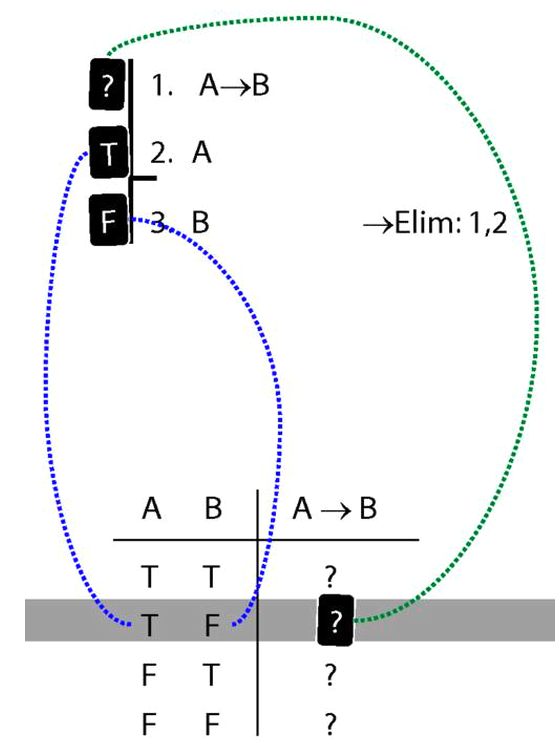
\includegraphics[scale=0.3]{img/unit_700_rule_to_tt.png}
\end{center}
 
 
\section{¬Elim}
 
\emph{Reading:} §6.3
 
\begin{center}
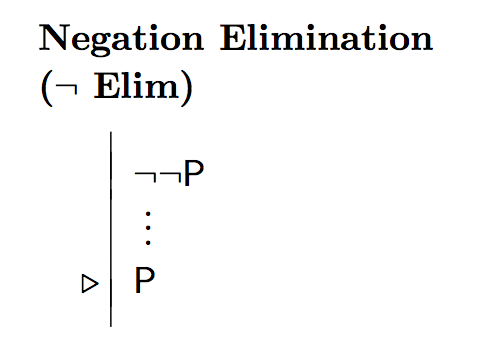
\includegraphics[scale=0.3]{img/rule_negation_elim.png}
\end{center}
 
 
\section{Scope: A Mistaken Application of ¬Elim}
 
What is wrong with this proof?
 
\begin{center}
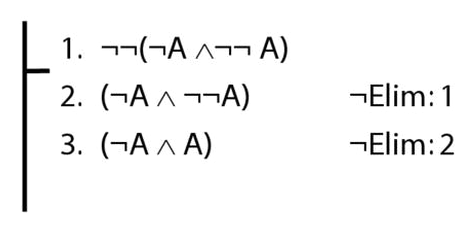
\includegraphics[scale=0.3]{img/proof_negation_elim_wrong.png}
\end{center}



\vfill


 
\section{¬Intro}
 
\emph{Reading:} §5.3, §6.3
 
\begin{center}
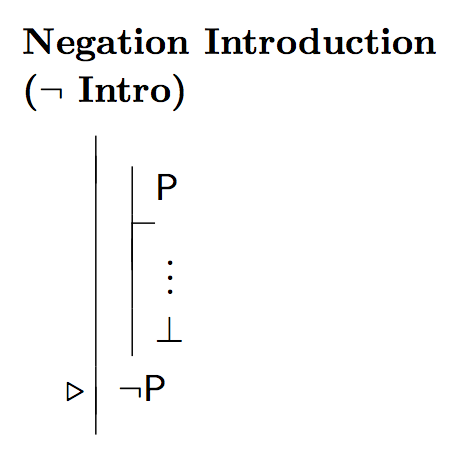
\includegraphics[scale=0.3]{img/rule_negation_intro.png}
\end{center}
\begin{center}
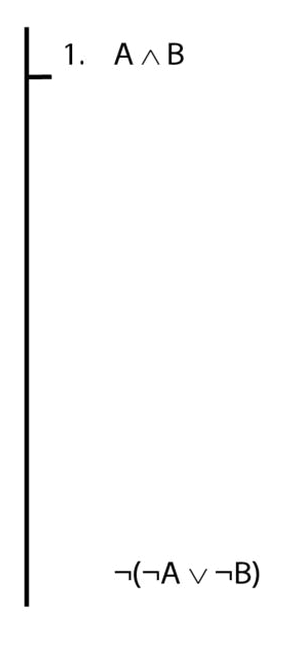
\includegraphics[scale=0.3]{img/proof_example_unit_281.png}
\end{center}



\vfill 
 
\section{A ∧ B ∨ C}
 
\emph{Reading:} §3.5
 
Ambiguity can be \emph{lexical}, e.g. `Actor testifies in horse suit'. Ambiguity can also be \emph{syntactic}, e.g. `How to combat the feeling of helplessness with illegal drugs'. (Both examples are from Bucaria, C. (2004), `Lexical and syntactic ambiguity as a source of humor: The case of newspaper headlines', Humour 17(3): 279--309.)
 
 
 
\section{A ∧ B ∨ C: They Are Different}
 
\begin{center}
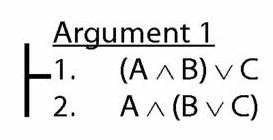
\includegraphics[scale=0.3]{img/arg1_unit_153.png}
\end{center}
\begin{center}
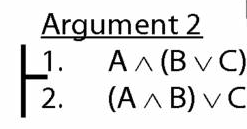
\includegraphics[scale=0.3]{img/arg2_unit_153.png}
\end{center}
 
 
\section{I Shot an Elephant in My Pyjamas}
 
Rule 1: a NP followed by a VP is a S
 
Rule 2: a Vt followed by a NP is a VP
 
Rule 3: a NP followed by a PP is a S
 
Rule 4: A Vt followed by a NP then a PP is a VP
 
Two derivations of Groucho Marx’ claim, ‘I shot an elephant in my pyjamas':
 
\begin{center}
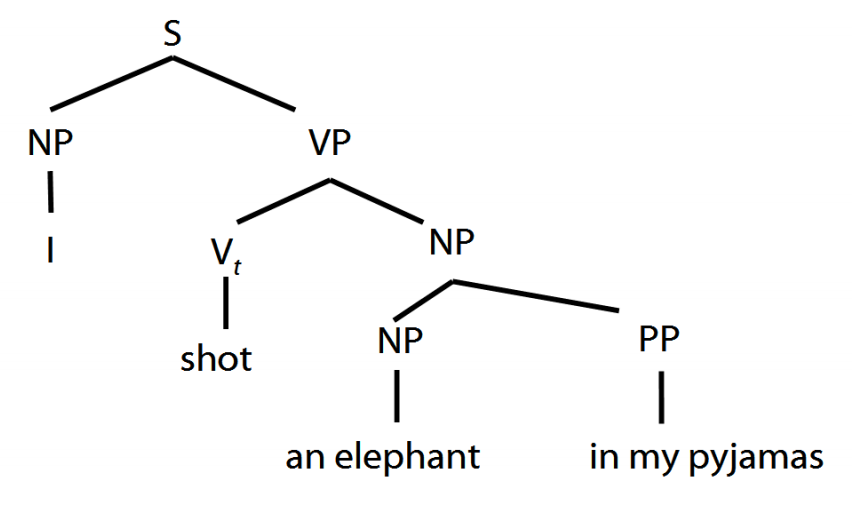
\includegraphics[scale=0.3]{img/groucho1.png}
\end{center}
\begin{center}
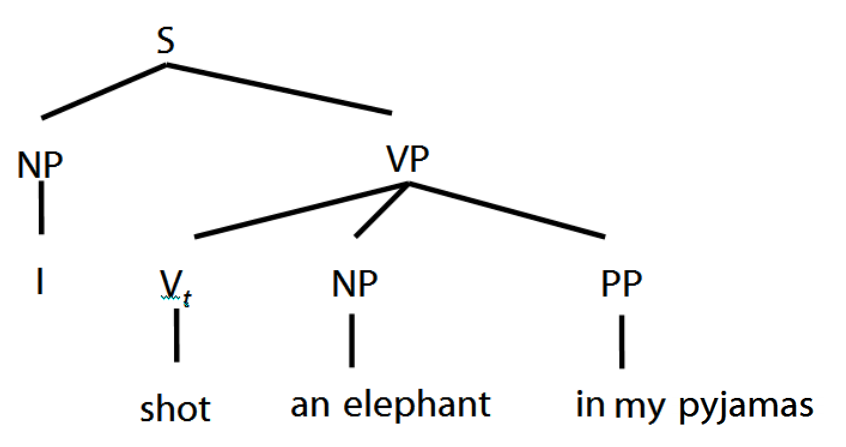
\includegraphics[scale=0.3]{img/groucho2.png}
\end{center}
 
 
\section{The Syntax of awFOL}
 
\emph{Reading:} §9.3
 
We define what counts as a sentence of awFOL using rules. E.g.:
 
1. If * and \# are sentences, then so is(* ∧ \#)
 
2. If * and \# are sentences, then so is (* ∨ \#)
 
3. P, Q, R, … are sentences
 
4. If * is a sentence, then ¬* is a sentence
 
So:
 
a. P is a sentence // rule 3
 
b. ¬P is a sentence // rule 4, a
 
c. ( ¬P ∧ Q ) is a sentence // rule 1, b, a
 
There is no structural ambiguity in awFOL because these rules are formulated to ensure that for any awFOL sentence, there is exactly one way of constructing it.
 
\begin{center}
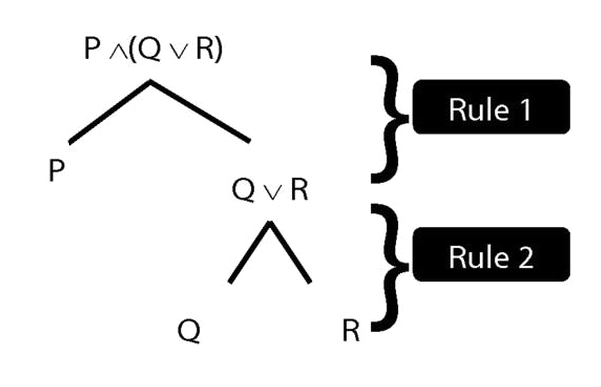
\includegraphics[scale=0.3]{img/unit_230_tree1.png}
\end{center}
\begin{center}
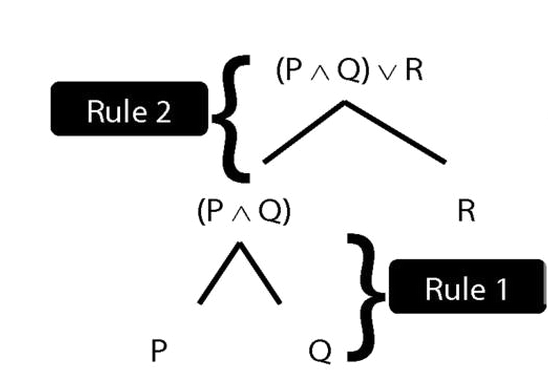
\includegraphics[scale=0.3]{img/unit_230_tree2.png}
\end{center}
\begin{center}
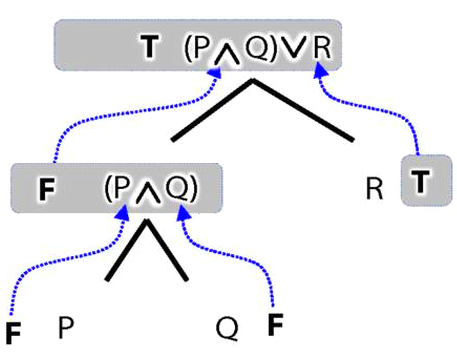
\includegraphics[scale=0.3]{img/unit_230_tree_tt.png}
\end{center}
 
 
\section{Scope: A Mistaken Application of ¬Elim}
 
What is wrong with this proof?
 
\begin{center}
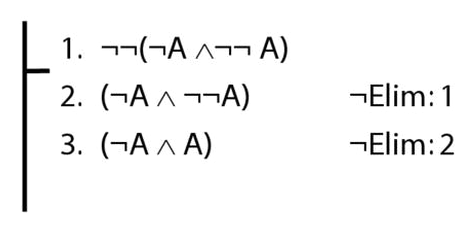
\includegraphics[scale=0.3]{img/proof_negation_elim_wrong.png}
\end{center}
 
 
\section{Scope}
 
\emph{Reading:} §3.5
 
The \emph{scope} of a connective (token) is the sentence containing it lowest in the tree.
 
\begin{center}
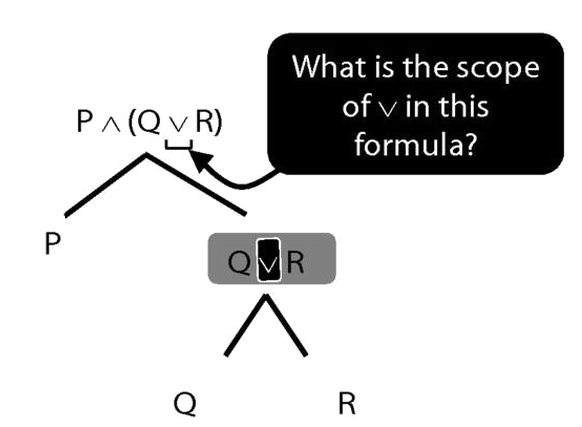
\includegraphics[scale=0.3]{img/unit_290_scope_q.png}
\end{center}
The connective with \emph{widest scope} is the one whose scope is the whole sentence.
 
\begin{center}
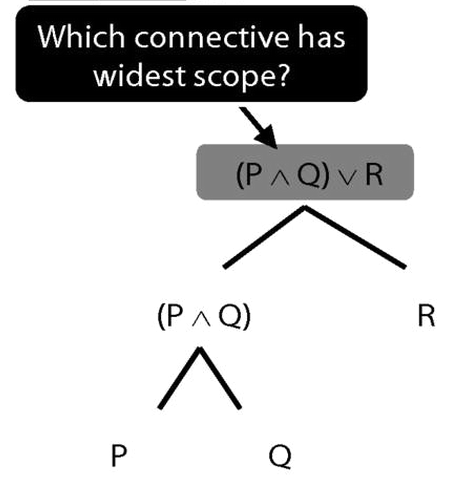
\includegraphics[scale=0.3]{img/unit_290_scope_q2.png}
\end{center}
A rule of proof can only be applied to the connective with widest scope.
 
\begin{center}
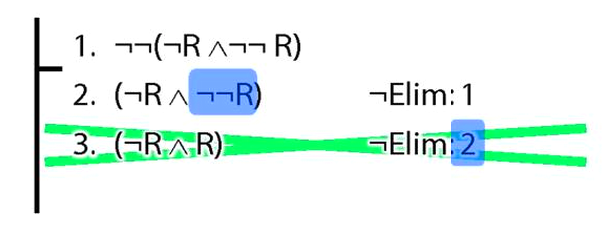
\includegraphics[scale=0.3]{img/unit_290_scope_proof.png}
\end{center}
When we do truth tables, the order we do the columns in is determined by scope.
 
\begin{center}
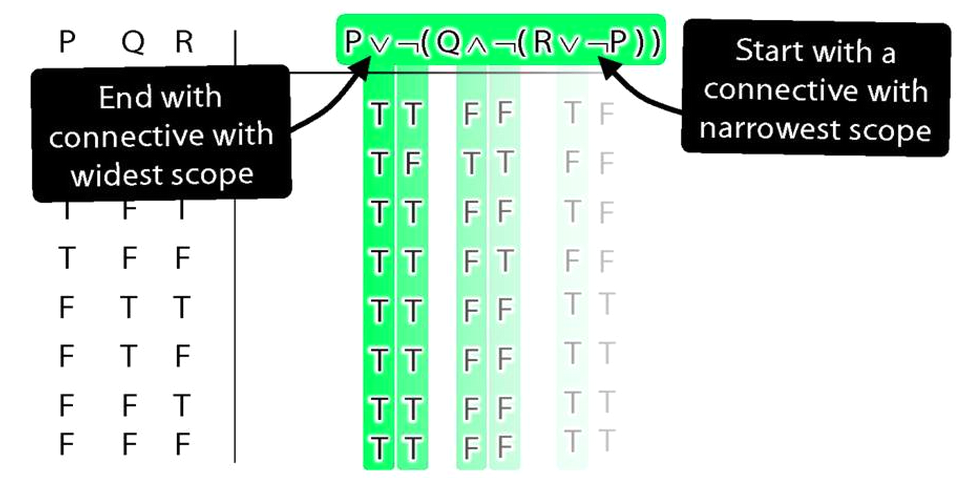
\includegraphics[scale=0.3]{img/unit_290_scope_tt.png}
\end{center}
 
 
\section{Truth-functional Connectives}
 
\emph{Reading:} §7.0 (the text before §7.1)
 
A \emph{connective} joins zero or more sentences to make a new sentence. Examples of connectives include: `∧', `¬', `$\bot$' and `because'.
 
A sentence joined by a connective is a \emph{constituent}. For example, consider the sentence ‘P because Q’: P is a constituent of this sentence.
 
A \emph{truth functional connective} produces a new sentence whose truth value depends only on the truth values of its constituent sentences.
 
When P and Q are both true, ‘P because Q’ is sometimes true and sometimes false. Therefore, ‘because’ is not a truth functional connective. To illustrate, consider `Alan got yellow cards because some apples are green' and `Alan got yellow cards because he used his elbows'. All the constituent sentences are true, but the first sentence is false whereas the second is true.
 
 
 
\section{Subproofs Are Tricky}
 
What is wrong with the following apparent proof?
 
\begin{center}
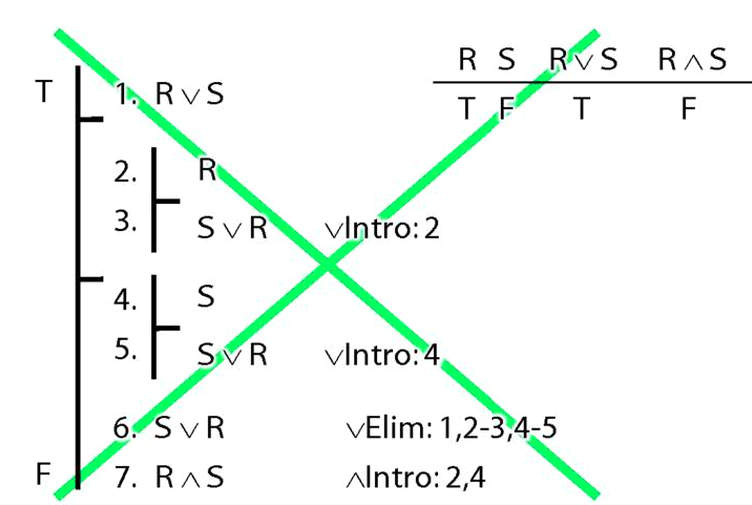
\includegraphics[scale=0.3]{img/unit_224_subproofs_tricky.png}
\end{center}
 
 
\section{Everything Is Broken}
 
\emph{Reading:} §9.1, §9.2
 
Everything is broken: ∀x Broken(x)
 
Something is broken: ∃x Broken(x)
 
%--- end paste
%--------------- 
 

\end{multicols*}

\end{document}